\documentclass[main.tex]{subfiles} 
\begin{document}

\section*{Teoretisk bakgrunn}
Gjennom underveisvurderingen følges elevenes progresjon
i faget over tid, og læreren får informasjon
om oppnådd kompetanse.

Det er ikke bare den faglige vurderingen som skal evalureres gjennom en skolegang. Ludvigsens utvalget mener
at den sosiale og emosjonelle utviklingen bør også ha større plass i vurderingsgrunnlaget enn det har idag :
\begin{displayquote}
Utvalget fremhever betydningen av et bredt kompetansebegrep,
og at skolen mer systematisk enn
i dag skal støtte elevenes sosiale og emosjonelle
læring og utvikling i fagene. For eksempel skal
elevene utvikle nysgjerrighet, selvregulering og
respekt for andres synspunkter. Sosiale og emosjonelle
kompetanser er ikke vektlagt systematisk
i dagens læreplaner, og det er derfor en endring
sammenlignet med i dag når dette blir en tydeligere
del av kompetansemålene i fagene. Dette
gir noen utfordringer som må håndteres på en
god måte i bestemmelser for vurdering og i lærernes
praksis. (NOU 2015: Fremtidens skole)
\end{displayquote}

Et prinsipp bør være at mål for elevenes sosiale
og emosjonelle kompetanse ikke tillegges vekt
i seg selv i den samlede sluttvurderingen, men at
de ses som forutsetninger for den kompetansen
elevene viser i faget.

\begin{figure}[h!]
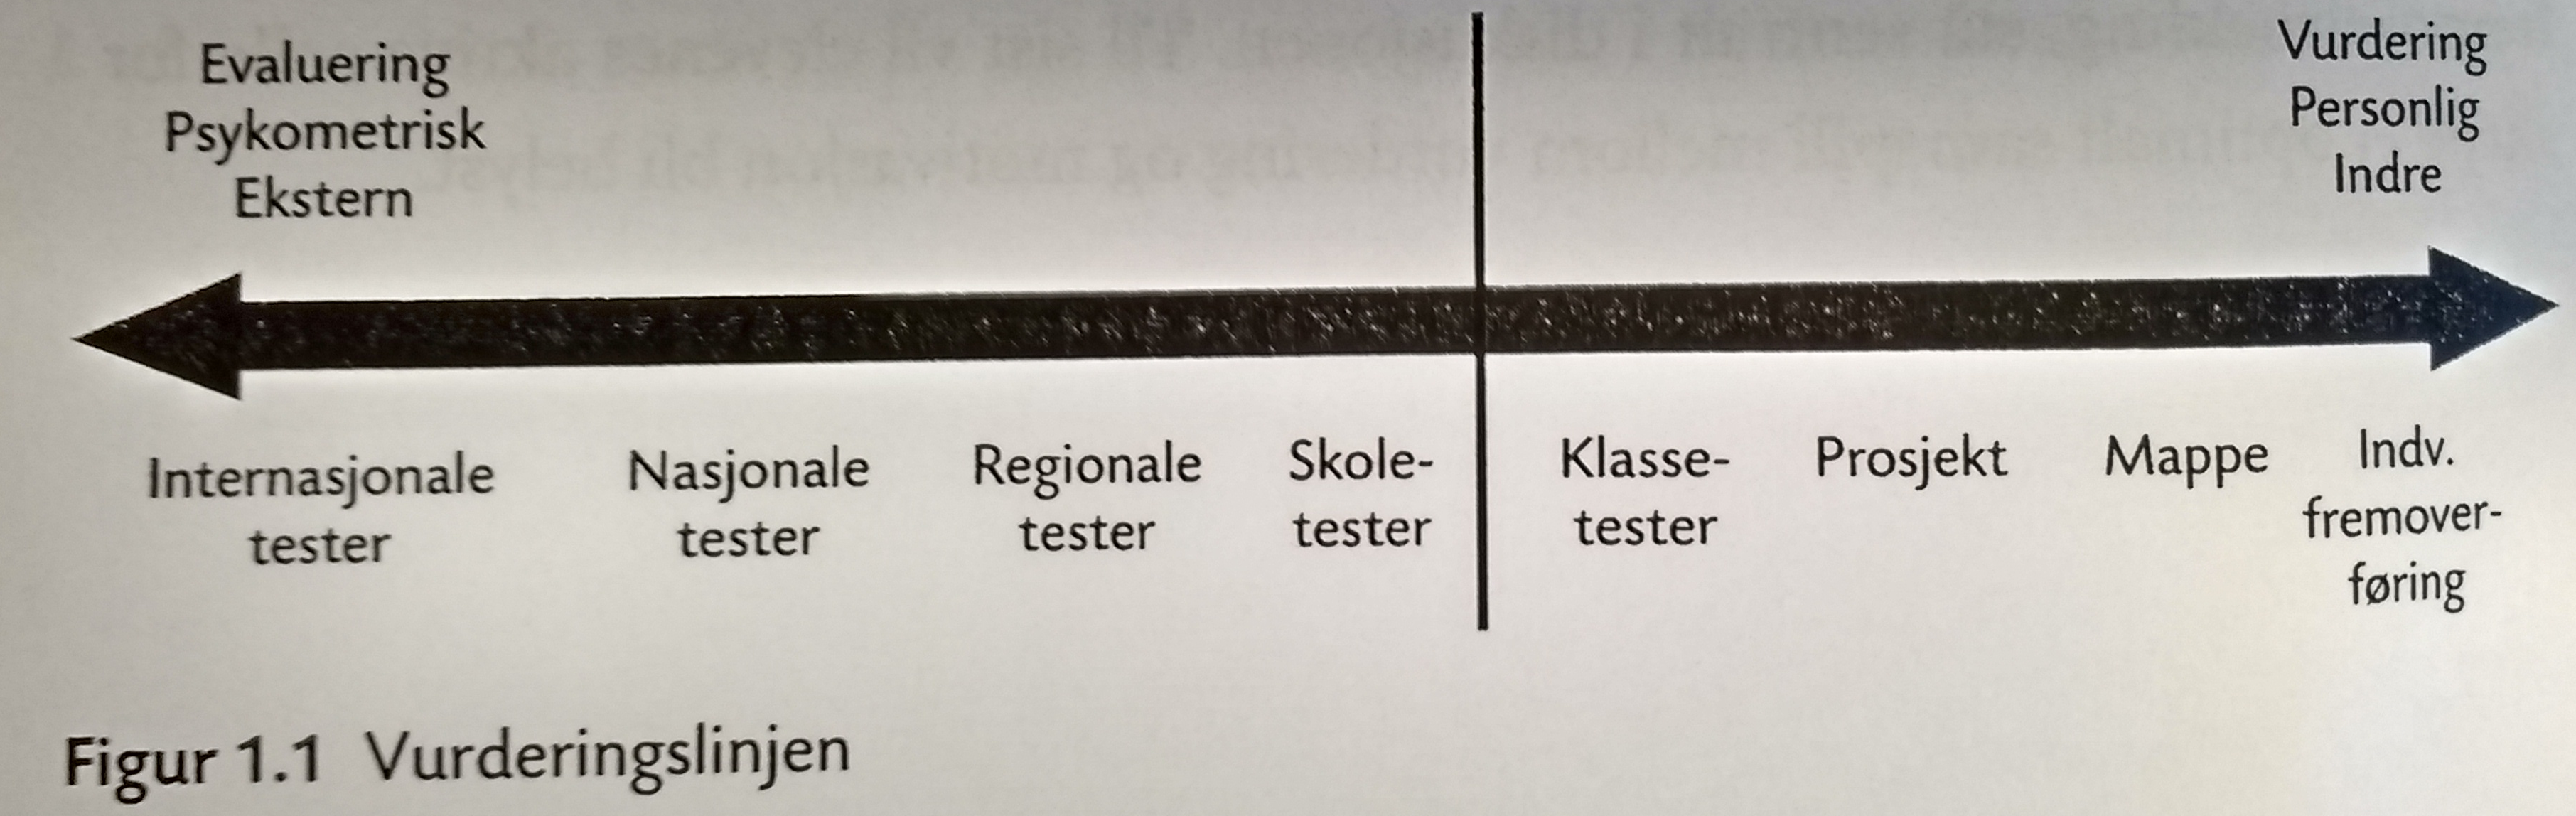
\includegraphics[scale = 0.1]{../figures/vurderingslinjen.png}
%\caption{Oversikt over naturfaglærernes undervisningstilbud til elevene fra PISA+ studie. Kilde: 
%\protect\citeA{odeg10}.}
%\label{fig:odeg10}
\end{figure}

Nordahl skriver at utfordringen er ikke at skolen mangler data, men at data ofte i lite grad blir
systematisk analysert og senere aktivt brukt for å forbedre praksisen (Nordahl, 2016).
\end{document}
